\begin{figure*}[htbp]
  \centering
  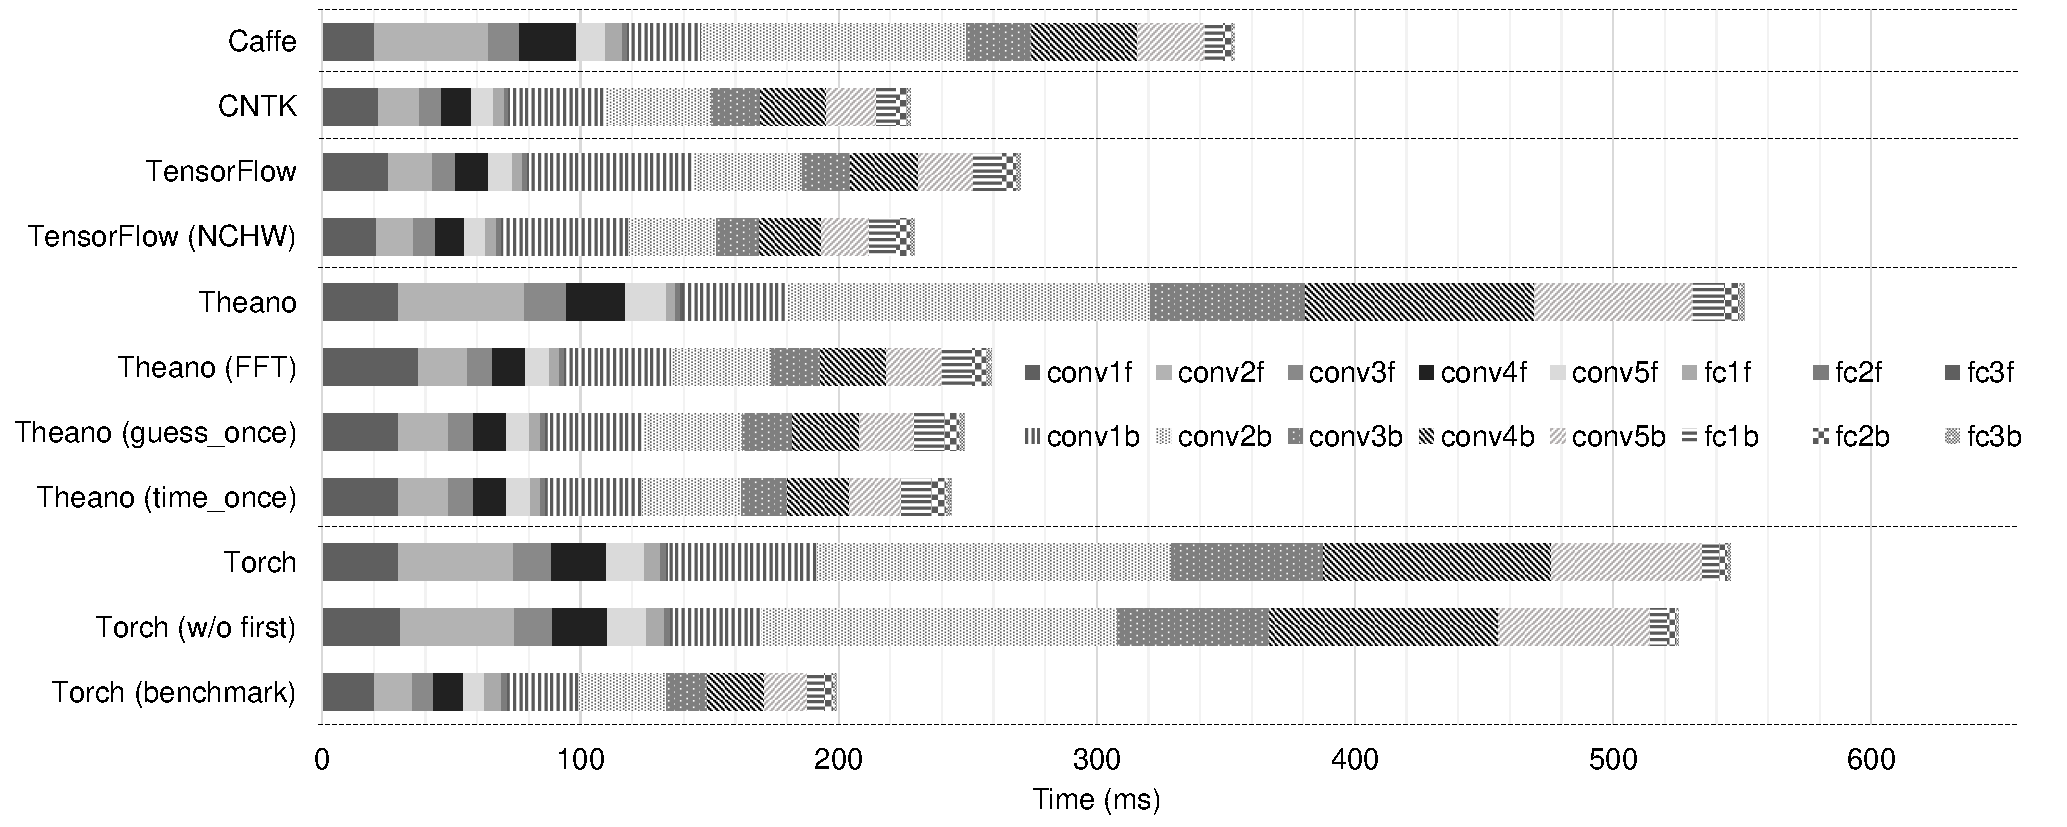
\includegraphics[width=\linewidth]{./figures/time_frameworks}
  \caption{%
The execution time of training AlexNet with a batch of imput images for differnt deep learning frameworks. 
\label{fig_time_frameworks}
  }
\end{figure*}

%A = Caffe, B = TensorFlow, C = TensorFlow (NCHW tensor), D = Theano, E = Theano (FFT), F = Theano (guess\_once), G = Theano (time\_once), H = Torch, I = Torch (no backward propagation in the first layer), J = Torch (FFT), K = Torch (benchmarking) 

\section{Charactrization on a Single GPU}
\label{sec:singlGPU}
In this section, we characterize the five deep learning frameworks on a single GPU. The measurement of the layer-wise execution time of AlexNet for each framework is shown in Figure~\ref{fig_time_frameworks}. The string in parantheses after the framework name stands for the configuration of the framework when AlexNet is built. No parantheses means the default options. A bar shows the breakdown of the total execution time in to that of each layer. A layer name suffixed with \textsf{f} stands for the forward computation phase, and \textsf{b} for the backward computation phase.

\subsection{Effect of GPU Kernel Implementations}
{\bf Caffe}. Caffe does not have any option to choose GPU kernels. Instead, it depends on cuDNN's heuristics that try to determine the best suited algorithm under the given specification. Surprisingly, Caffe does not have an appropriate memory management technique yet. It just passes the 8MB workspace limit as an argument to the GPU kernel. As result, algorithms that require low memory, such as GEMM and Winograd, are unappropriately selected resulting in low performance even if Caffe exploits cuDNN's heuristics. 

{\bf TensorFlow}. TensorFlow also does not provide options for GPU kernel choices. Unlike Caffe, however, it executes all available algorithms in the first run by itself. Then, the fastest GPU kernel in each layer is executed in subsequent runs. The FFT algorithm is chosen for all the convolution layers except the first layer, where FFT cannot be used because of the stride size (4). Since the set of algorithms that can be chosen is fixed and hardwired, a recently added option WINOGRAD\_NONFUSED cannot be included in the set.

{\bf Theano}. On the other hand, Theano provides full accesses on the GPU kernel choices. Users can specify a specific convolution algorithm globally or in a layer-by-layer manner. There are two types of GPU GEMM kernels in Theano: explicit and implicit. The default is the explicit GEMM. When a global convolution algorithm is given, and the GPU kernel for the algorithm does not match the condition for a layer specified by Theano, the implicit GEMM is chosen as a fallback for the layer. However, the implicit GEMM is usually slower than the explicit GEMM. Thus, it is better to give layerwise option to avoid choosing the implicit GEMM. \Comment{$<$==== Check this! ===} 

This is the reason why the first layer of \textsf{Theano (FFT)} in Figure~\ref{fig_time_frameworks} is slower than \textsf{Theano (guess\_once)}, \textsf{Theano (time\_once)}, and even \textsf{Theano}. The \textsf{guess\_once} option makes Theano behaves like Caffe where cuDNN's heuristics determine the best suited algorithm. Unlike Caffe, it properly exploits cuDNN's heuristics when the \textsf{guess\_once} option is given\Comment{$<$==== Check this! ===} 

The \textsf{time\_once} option in Theano exploits cuDNN's another functionality that executes all available convolution algorithms and choose the fastest one. Unlike TensorFlow, the set of algorithms is not hardwired. Instead, Theano directly uses cuDNN's API functions.

When \textsf{time\_once} option is on, Theano uses GEMM in the first layer. In the rest of the convolution layers, it uses FFT or Winograd. The \textsf{guess\_once} option is on, the usage of GPU kernels is slightly different but their execution time is almost the same as that of \textsf{time\_once}.
This implies that cuDNN's heuristics are quite reliable.

\begin{table}[htbp]
\centering
\caption{Other GPU Kernels}
\label{table_misc_kernel}
\begin{scriptsize}
\begin{tabular}{|l|l|l|l|l|l|}
\hline\hline
GPU kernel & Caffe    & CNTK & TensorFlow & Theano  & Torch \\ \hline\hline
Bias       & cuDNN    &      & TensorFlow & Theano  & cuDNN \\ \cline{2-6} 
addition   & 2.64 ms  &      & 2.84 ms    & 7.88 ms & 2.63 ms  \\ \hline\hline
ReLU       & cuDNN    &      & Eigen      & Theano  & cuDNN \\ \cline{2-6}
activation & 2.56 ms  &      & 2.43 ms    & 4.59 ms & 2.56 ms  \\ \hline
\end{tabular}
\end{scriptsize}
\end{table}

Although Theano executes the fastest GPU kernels for convolution computation, it does have the fastest convolution layers because of other GPU kernels for bias addition and ReLU activation. Table~\ref{table_misc_kernel} lists the GPU kernels included in a convolution layer, but not directly participates in convolution computation. It also shows the source of the GPU kernels. The execution time of the GPU kernels is measured in the first convolution layer. Since Theano uses GPU kernels that are dynamically compiled at run time, they are noticeably slower than those in other frameworks.

{\bf Torch}. Like Theano, Torch provides a full control over GPU kernel choices. Its cuDNN backend, cudnn.torch, has \textsf{cudnn.benchmark} option that is the same as \textsf{time\_once} in Theano. When \textsf{benchmark} option is on, Torch is the fastest. 

\subsection{Effect of Data Layout}
We also find that data layout affects performance a lot. The most noticable one is the tensor format.
Caffe, Theano, and Torch use the $NCHW$ 4D tensor format mentioned in Section~\ref{sec:CNN}. When $N$, $C$, $H$, and $W$ are the number of images in a batch, the number of channels, the height of a feature map, and the width of a feature map, respectively, the $NCHW$ 4D tensor data are stored in the order of the dimensions $N$, $C$, $H$, and $W$. 

Even though TensorFlow supports the $NCHW$ format, it seems to prefer the $NHWC$ format. Sample code in TensorFlow uses the $NHWC$ format, and many functions in TensorFlow, such as conv2d, uses it as a default argument. Since channel data are stored in the last dimension in the $NHWC$ format, the performance will be better off using it when there are innermost channel-wise operations. However, some convolution kernels, such as FFT, in cuDNN supports only $NCHW$ format. Moreover, by default, TensorFlow performs conversion between $NHWC$ and $NCHW$ even if it uses GPU kernels that support the $NHWC$ format. Thus, using the $NHWC$ tensor format introduces significant conversion overhead before and after a convolution. In Figure~\ref{fig_time_frameworks}, just changing the tensor format from $NHWC$ to $NCHW$ leads to about 15\% performance improvement. 

\subsection{Redundant Backward Propagation}
The first convolution layer in AlexNet does not have its previous layer. Thus, there is no need to perform the back propagation of gradients computed in the first layer. Caffe and Theano automatically omit the back propagation. Torch omits it when \textsf{gradInput} of the first layer is set to nil. \Comment{$<$=== Check this! ===}

On the contrary, TensorFlow always perform the back propagaton of the first layer to prevent non-reproducibility caused by race conditions (gate\_gradients parameter in tf.train.Optimizer.compute\_gradients). This makes TensorFlow slower than Torch even if Torch has almost the same GPU kernels as those of TensorFlow. For this reason, in Figure~\ref{fig_time_frameworks}, we see that the execution time of \textsf{conv1b} in \textsf{TensorFlow (NCHW)} is significantly different from that in \textsf{Torch (benchmark)}. \Comment{$<$==== Check it! ===} 

However, it can be disabled at the expense of reproducibility and the accuracy of gradient computation, although we left it enabled in our experiment for Figure~\ref{fig_time_frameworks}.

Based on the above observations, we can increase the speed of training a CNN model up to twice by just changing options in a framework. We do not need to modify the source code of the framework at all. For example, \textsf{Theano (FFT)}, \textsf{Theano (guess\_once)}, and \textsf{Theano (time\_once)} are twice faster than \textsf{Theano}, \textsf{Torch (FFT)} and \textsf{Torch (benchmark)} are also twice faster than \textsf{Torch}. 

%그 외 사소한 것으로 텐서에 네트워크 입력을 feed_dict로 주면 CPU 복사가 일어나서 매우 느리므로 FixedLengthRecordReader 등으로 주는게 좋다.
%https://github.com/tensorflow/tensorflow/issues/2919

%https://github.com/BVLC/caffe/blob/rc3/src/caffe/layers/cudnn_conv_layer.cpp#L113
%https://github.com/tensorflow/tensorflow/blob/v0.10.0rc0/tensorflow/core/kernels/conv_ops.cc#L460
%https://github.com/tensorflow/tensorflow/blob/v0.10.0rc0/tensorflow/stream_executor/cuda/cuda_dnn.cc#L933
%https://github.com/Theano/Theano/blob/rel-0.8.2/theano/sandbox/cuda/dnn.py#L285
%https://github.com/Theano/Theano/blob/rel-0.8.2/theano/sandbox/cuda/dnn_fwd.c#L227
%https://github.com/soumith/cudnn.torch/blob/R5/SpatialConvolution.lua#L166

